\section{Module 4. Non-stationary noise filtering 1}

Linear minimum mean square error method consist of three step:

\begin{itemize}
\item Estimate the second or fourth order moment
\item Calculate the K parameter
\item Estimate new signal without noise
\end{itemize}

The code was prepered in simens class template. The main programme is diveded to part of code for structural data and diffusion data. The data, which is received, includes whole set of brain slices. The structural data has three dimensions - first two dimensions are the number of pixels in MR image. The third includes the number of slices. The LMMSE filter is called for every slice in whole data set. Diffusion data has one more dimension, which described the number of diffusion gradients. The LMMSE filter is called also for every slice and every diffusion gradients. In this data is used one more for loop to iterate data by every number of gradient.

Module is divided into two functions and one main function. One of them is prepered to estimate the second and the fourth order moment.The second function includes estimatin new image and calculating K parameter. K-th order moment is calculated using the estimator of k-th raw sample moment for two-dimensional data: 
\begin{equation}
\begin{aligned}\langle I_{ij}^k\rangle=\frac{1}{|\eta_{ij}|}\sum\limits_{p\epsilon\eta_{ij}} I_p^k \end{aligned}
\label{m4Im1}
\end{equation}
This case is solved by convolution data with sqaure neighbourhood divided by size of the window. The size of neihbourhood window is chosen experimentally. We used the python function \emph{convolve2d}, which convolve two 2-dimensional arrays with output size determined by mode. The mode is checked to 'same', because we need the same size of arrays. The inputs of first function are image and square neighbourhood window, the function return second and fourth order moment (two-dimensional array).

Next step is to calculate the K parameter, which is defined:
\begin{equation}
\begin{aligned}K_{ij}^{2}=1-\frac{4\sigma_{n}^{2}(\langle M_{i}j^{2}\rangle-2\sigma_{n}^{2})}{\langle M_{i}j^{4}\rangle-{\langle M_{i}j^{2}\rangle}^{2}}\end{aligned}
\label{m4Im2}
\end{equation}
With numpy array we could easily perform transformations on arrays without using loops. 

The last step of programme is estimated new image without noise. The estimator is defined:
\begin{equation}
\begin{aligned}\widehat{A_{ij}^{2}}=\langle M_{i}j^{2}\rangle-2\sigma_{n}^{2}+K_{ij}(M_{ij}^{2}-\langle M_{ij}^{2}\rangle)\end{aligned}
\label{m4Im3}
\end{equation}
After estimation $A_{ij}^2$, we calculate the absolute value pixels in the new image, beacuse we need positive value to sqaure root. Then, we calculate the positive square-root of an array. The inputs of second function are image, noise map and square neighbourhood window, the function return new, estimated image without noise. The result of main function is returned to next module as class.

The programme is really fast, the duration time is approximately 0.046 second for one image.
To improve working of method, we checked the different size of sqaure neihbourhood window to adjust it to receive the best results. To compare result we used the relative error:
\hfill{}\\

\begin{tabular}{c r @{,} l}
Window &
\multicolumn{2}{c}{Relative error}\\ \hline
3 & 0&07 \\
4 & 0&02 \\
5 & 0&005 \\
6 & 0&002 \\
7 & 0&011 \\
10 & 0&014 \\

\end{tabular}
\hfill{}\\


The best result for filtering image is when window size equals 6. When the size is higher than 6 the good filtering results is occurs in background of image, but noise appears in the contour of brain.

\begin{figure}[H]
\centering{}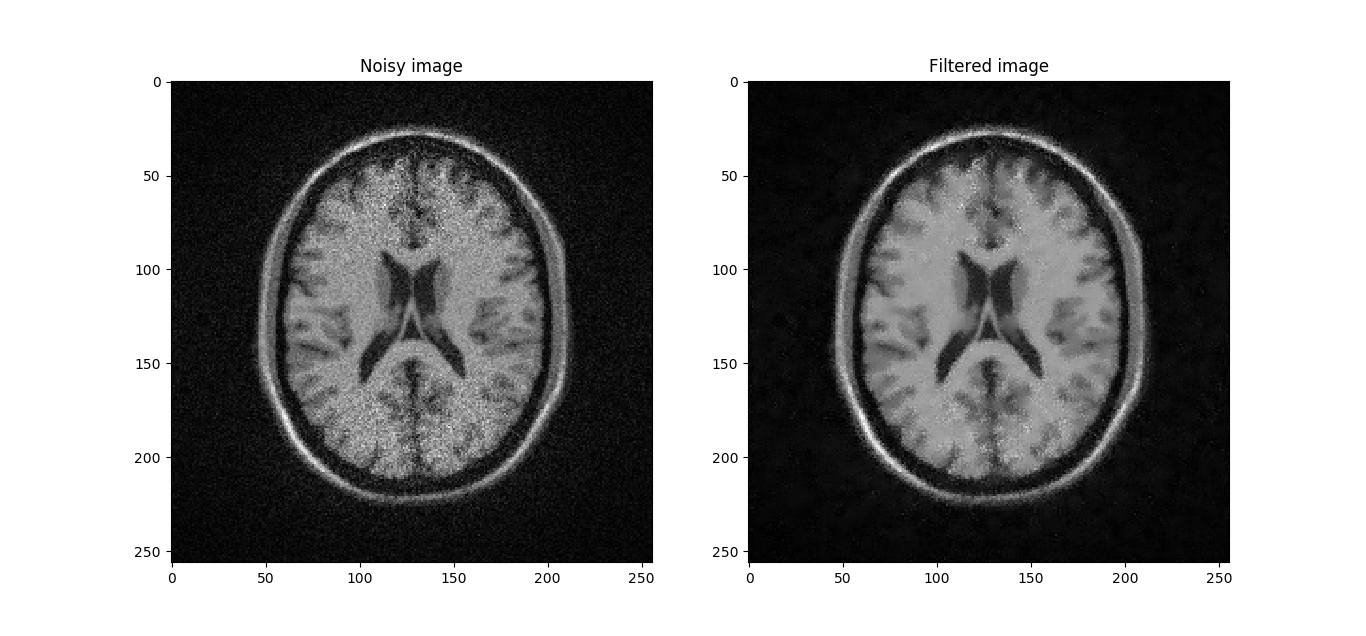
\includegraphics[scale=0.3]{figures/Module_4/LMMSE_test_win6}\caption{Results of LMMSE estimation with size window equal 6} \label{fig:figures/Module_4/LMMSE_test_win6}
\end{figure}

\begin{figure}[H]
\centering{}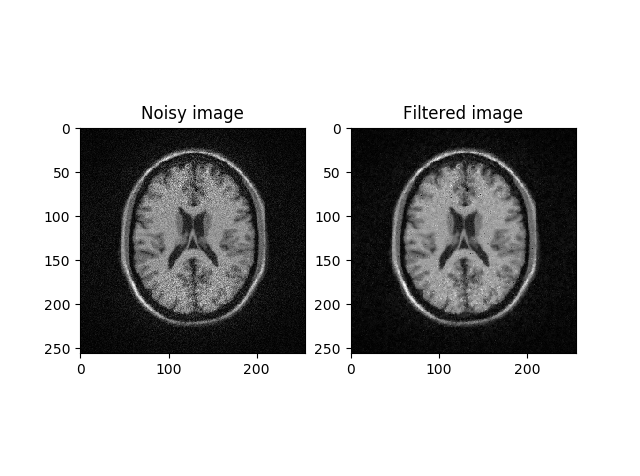
\includegraphics[scale=0.7]{figures/Module_4/LMMSE_test_win3}\caption{Results of LMMSE estimation with size window equal 3} \label{fig:figures/Module_4/LMMSE_test_win3}
\end{figure}

\begin{figure}[H]
\centering{}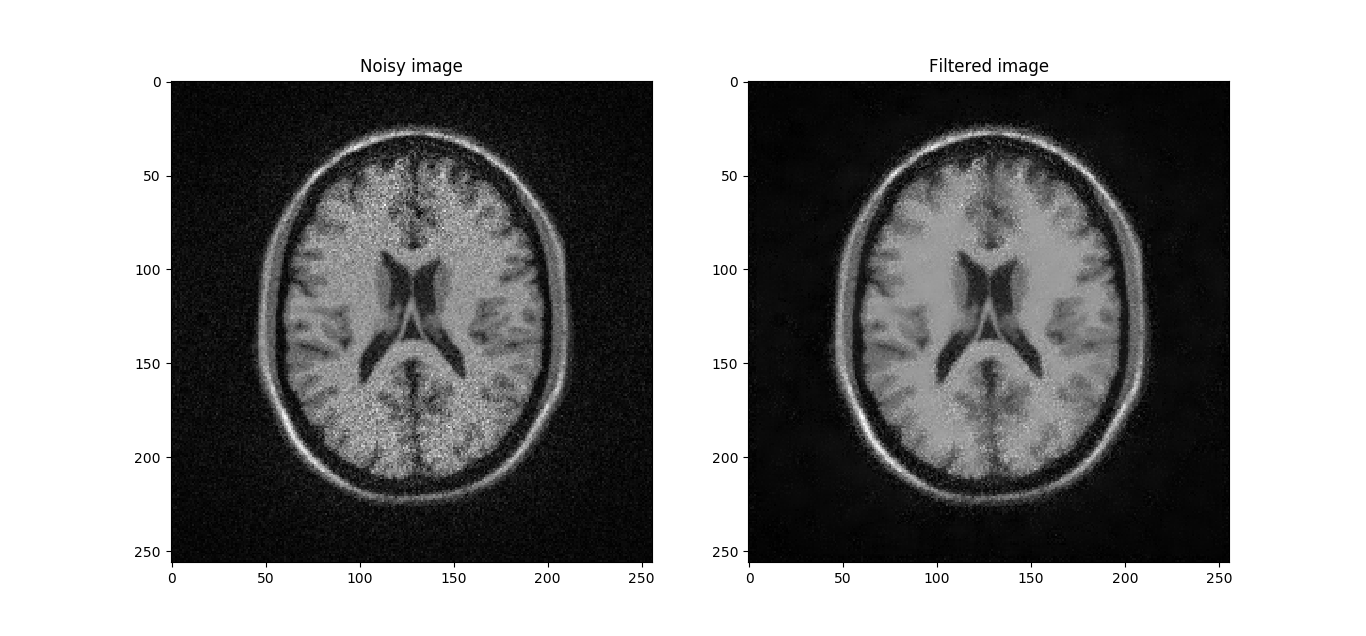
\includegraphics[scale=0.3]{figures/Module_4/LMMSE_test_win10}\caption{Results of LMMSE estimation with size window equal 10} \label{fig:figures/Module_4/LMMSE_test_win10}
\end{figure}